% !TEX TS-program = XeLaTeX
% use the following command:
% all document files must be coded in UTF-8
\documentclass[english]{textolivre}
% build HTML with: make4ht -e build.lua -c textolivre.cfg -x -u article "fn-in,svg,pic-align"

\journalname{Texto Livre}
\thevolume{19}
%\thenumber{1} % old template
\theyear{2026}
\receiveddate{\DTMdisplaydate{2025}{12}{1}{-1}} % YYYY MM DD
\accepteddate{\DTMdisplaydate{2026}{2}{4}{-1}}
\publisheddate{\DTMdisplaydate{2026}{4}{13}{-1}}
\corrauthor{Mu You}
\articledoi{10.1590/1983-3652.2026.63188}
%\articleid{NNNN} % if the article ID is not the last 5 numbers of its DOI, provide it using \articleid{} commmand 
% list of available sesscions in the journal: articles, dossier, reports, essays, reviews, interviews, editorial
\articlesessionname{dossier}
\runningauthor{You et al.} 
%\editorname{Leonardo Araújo} % old template
\sectioneditorname{Zaira Bomfante dos Santos~\orcid{0000-0002-6162-8489}}
\layouteditorname{Leonardo Araújo~\orcid{0000-0003-3884-2177}}

\title{Exploring learner prompting and AI feedback quality in L2 Portuguese writing}
\othertitle{Explorando o uso de prompts por aprendizes e a qualidade do feedback de IA na escrita em português como segunda língua}
% if there is a third language title, add here:
%\othertitle{Artikelvorlage zur Einreichung beim Texto Livre Journal}

\author[1]{Mu You~\orcid{0000-0001-5029-3903}\thanks{Email: \href{youmuafonso@gmail.com}{youmuafonso@gmail.com}}}
\author[2]{Jing Zhang~\orcid{0000-0003-4801-6354}\thanks{Email: \href{jingz@um.edu.mo}{jingz@um.edu.mo}}}
\author[2]{Chunhui Lu~\orcid{0000-0001-7744-9197}\thanks{Email: \href{luchunhui@um.edu.mo}{luchunhui@um.edu.mo}}}
\author[3]{Ana Cristina Ferreira de Almeida Rodrigues Alves~\orcid{0000-0002-1461-4746}\thanks{Email: \href{anacristinaalves@cccm.gov.pt}{anacristinaalves@cccm.gov.pt}}}
\author[4]{Jiaxu Zuo~\orcid{0009-0009-9950-3348}\thanks{Email: \href{mc45440@um.edu.mo}{mc45440@um.edu.mo}}}
\affil[1]{Macau Millennium College, Institute of International Language Services Studies, Macau SAR, China.}
\affil[2]{University of Macau, Faculty of Arts and Humanities, Department of Portuguese, Macau SAR, China.}
\affil[3]{Macau Scientific and Cultural Centre, Lisbon, Portugal.}
\affil[4]{University of Macau, Faculty of Science and Technology, Department of Computer and Information Science, Macau SAR, China.}

\addbibresource{article.bib}
% use biber instead of bibtex
% $ biber article

% used to create dummy text for the template file
\definecolor{dark-gray}{gray}{0.35} % color used to display dummy texts
\usepackage{lipsum}
\SetLipsumParListSurrounders{\colorlet{oldcolor}{.}\color{dark-gray}}{\color{oldcolor}}

% used here only to provide the XeLaTeX and BibTeX logos
\usepackage{hologo}

% if you use multirows in a table, include the multirow package
\usepackage{multirow}
\usepackage[UTF8]{ctex}  % 支持中文
\usepackage{graphicx}
\usepackage{amsmath}
% provides sidewaysfigure environment
\usepackage{rotating}
% CUSTOM EPIGRAPH - BEGIN 
%%% https://tex.stackexchange.com/questions/193178/specific-epigraph-style
\usepackage{epigraph}
\renewcommand\textflush{flushright}
\makeatletter
\newlength\epitextskip
\pretocmd{\@epitext}{\em}{}{}
\apptocmd{\@epitext}{\em}{}{}
\patchcmd{\epigraph}{\@epitext{#1}\\}{\@epitext{#1}\\[\epitextskip]}{}{}
\makeatother
\setlength\epigraphrule{0pt}
\setlength\epitextskip{0.5ex}
\setlength\epigraphwidth{.7\textwidth}
% CUSTOM EPIGRAPH - END

% LANGUAGE - BEGIN
% ARABIC
% for languages that use special fonts, you must provide the typeface that will be used
% \setotherlanguage{arabic}
% \newfontfamily\arabicfont[Script=Arabic]{Amiri}
% \newfontfamily\arabicfontsf[Script=Arabic]{Amiri}
% \newfontfamily\arabicfonttt[Script=Arabic]{Amiri}
%
% in the article, to add arabic text use: \textlang{arabic}{ ... }
%
% RUSSIAN
% for russian text we also need to define fonts with support for Cyrillic script
% \usepackage{fontspec}
% \setotherlanguage{russian}
% \newfontfamily\cyrillicfont{Times New Roman}
% \newfontfamily\cyrillicfontsf{Times New Roman}[Script=Cyrillic]
% \newfontfamily\cyrillicfonttt{Times New Roman}[Script=Cyrillic]
%
% in the text use \begin{russian} ... \end{russian}
% LANGUAGE - END

% EMOJIS - BEGIN
% to use emoticons in your manuscript
% https://stackoverflow.com/questions/190145/how-to-insert-emoticons-in-latex/57076064
% using font Symbola, which has full support
% the font may be downloaded at:
% https://dn-works.com/ufas/
% add to preamble:
% \newfontfamily\Symbola{Symbola}
% in the text use:
% {\Symbola }
% EMOJIS - END

% LABEL REFERENCE TO DESCRIPTIVE LIST - BEGIN
% reference itens in a descriptive list using their labels instead of numbers
% insert the code below in the preambule:
%\makeatletter
%\let\orgdescriptionlabel\descriptionlabel
%\renewcommand*{\descriptionlabel}[1]{%
%  \let\orglabel\label
%  \let\label\@gobble
%  \phantomsection
%  \edef\@currentlabel{#1\unskip}%
%  \let\label\orglabel
%  \orgdescriptionlabel{#1}%
%}
%\makeatother
%
% in your document, use as illustraded here:
%\begin{description}
%  \item[first\label{itm1}] this is only an example;
%  % ...  add more items
%\end{description}
% LABEL REFERENCE TO DESCRIPTIVE LIST - END


% add line numbers for submission
%\usepackage{lineno}
%\linenumbers

\begin{document}
\maketitle

\begin{polyabstract}


\begin{abstract}
For L2 Portuguese learners in Macau, artificial intelligence (AI) has become a primary source of immediate writing feedback for Chinese university students. This study investigates authentic learner prompting practices and the accuracy of resulting AI-generated revisions in L2 Portuguese writing. Forty-six second-year Portuguese Studies majors, divided into a control condition and a justification condition that required them to rationalize every modification, revised a first-year learner composition using their preferred AI tools. Results reveal that students predominantly prompted in Chinese, employed highly anthropomorphic and polite language, relied on generic or grammar-focused requests, and frequently exhibited misalignment between intended goals and actual prompts. The requirement to justify revisions increased interaction turns and shifted attention toward smaller textual units and explanation-seeking, though it also produced higher error rates in the resulting revisions. Experiments with researcher-designed prompts demonstrated the potential of simple prompt engineering strategies, with the Rephrase-and-Respond technique eliciting the most accurate revisions. The findings underscore the immaturity of untrained prompting, the context-sensitive nature of prompt engineering, and the practical pedagogical value of current LLMs even under naïve use. To foster critical and reflective human–AI collaboration in L2 writing, pedagogical interventions such as explicit instruction in prompting strategies and the use of tasks that require justification or explanation-seeking are recommended.


\keywords{AI-assisted writing revision \sep Prompting behavior \sep Revision accuracy \sep L2 Portuguese}
\end{abstract}

\begin{portuguese}
\begin{abstract}
Para aprendizes de Português como L2 em Macau, a inteligência artificial (IA) tornou-se uma fonte principal de \textit{feedback} imediato na escrita para estudantes universitários chineses. Este estudo investiga as práticas autênticas de \textit{prompting} dos aprendizes e a precisão das revisões geradas por IA na escrita em português L2. Quarenta e seis estudantes do segundo ano da licenciatura em Estudos Portugueses, divididos num grupo de controle e num grupo com condição de justificação (que exigia que racionalizassem cada alteração), revisaram uma composição de uma estudante do primeiro ano utilizando as suas ferramentas de IA preferidas. Os resultados revelam que os estudantes utilizaram predominantemente o chinês nos \textit{prompts}, empregaram linguagem altamente antropomórfica e cortês, recorreram a pedidos genéricos ou centrados na gramática e, frequentemente, apresentaram desalinhamento entre os objetivos pretendidos e os \textit{prompts} efetivamente formulados. A obrigatoriedade de justificar as revisões aumentou o número de turnos de interação e deslocou a atenção para segmentos textuais mais reduzidos e para a busca de explicações, embora também tenha gerado taxas de erro mais elevadas nas revisões. Experiências com \textit{prompts} desenhados pelos investigadores demonstraram o potencial de estratégias simples de engenharia de \textit{prompt}, sendo a técnica \textit{Rephrase-and-Respond} a que produziu as revisões mais precisas. Os resultados sublinham a imaturidade do \textit{prompting} não treinado, a natureza sensível ao contexto da engenharia de \textit{prompt} e o valor pedagógico prático das atuais ferramentas de IA mesmo quando usados sem treinamento prévio. Para promover uma colaboração humano–IA crítica e reflexiva na escrita em L2, recomendam-se intervenções pedagógicas como a instrução explícita em estratégias de \textit{prompting} e a utilização de tarefas que exijam justificação ou busca de explicações.

\keywords{Revisão de escrita assistida por IA \sep Comportamento de \textit{prompting} \sep Precisão das revisões \sep Português L2}
\end{abstract}
\end{portuguese}

% if there is another abstract, insert it here using the same scheme
\end{polyabstract}

\section{Introduction}\label{sec-intro}

The transformative impact of artificial intelligence (AI) on education has intensified dramatically in recent years, reshaping how students approach second language (L2)\footnote{In this paper, ``L2'' is used as an umbrella term for non-native language.} learning, especially writing \cite{BARROT2023100745,crompton2023,Kohnke2023,lo2023,Luo2025}. In Macau, a Special Administrative Region of China where Portuguese retains official status yet is spoken natively by only approximately 2.3\% of the population\footnote{See \href{https://www.dsec.gov.mo/getAttachment/fda23546-c321-47ae-a5b3-b4a5071cf732/P_CEN_PUB_2021_Y.aspx}{the Macau official census statistics of 2021.}}, opportunities for authentic interaction in Portuguese outside the university classroom are limited. For the Chinese university students learning L2 Portuguese, large language models (LLMs) have become the most accessible, immediate, and relatively reliable source of feedback on written production. These tools enable students to refine their compositions independently, reducing dependence on scarce and often unavailable human tutors or native-speaker peers beyond formal instructional settings.

This reliance on AI is corroborated by a preliminary survey administered to 46 second-year Portuguese Studies majors at a Macau university. 44 respondents (95.7\%) reported daily use of AI tools, and the most popular platforms were DeepSeek (71.7\%), Doubao (54.3\%), ChatGPT (28.3\%), Copilot (17.4\%), and Kimi (13.0\%) (multiple selections allowed). Writing revision, alongside general knowledge queries, emerged as the dominant primary purpose, reported by 37 students (80.4\%). These data confirm that AI has assumed a central role in the L2 Portuguese writing development of this learner population. 

Despite the widespread adoption, both typical student prompting behaviors in this context, and the quality of the resulting AI-generated revisions remain underexplored \cite{hwang2024exploring}. This gap motivates four interrelated research questions: 

    \textbf{RQ\#1}: How do learners actually prompt AI systems when seeking writing revision in an L2 Portuguese context?

    \textbf{RQ\#2}: What is the accuracy of AI-generated revisions under authentic, student-initiated prompting conditions?

    \textbf{RQ\#3}: How does requiring learners to provide revision rationales affect their prompting behavior and the accuracy of AI-generated feedback?
    
    \textbf{RQ\#4}: To what extent can simple prompt-engineering techniques improve the accuracy of AI-generated revisions compared to typical student prompts?


Learner prompting is inherently variable rather than standardized. Given that prompt formulation is known to significantly affect AI output quality \cite{sahoo2025,2024schulho}, the feedback students ultimately receive can vary considerably in linguistic accuracy. Empirical investigation is therefore essential to describe authentic prompting practices \textbf{(RQ\#1)}, evaluate the real-world reliability of AI-generated revisions \textbf{(RQ\#2)}, and determine whether modest interventions in task requirement \textbf{(RQ\#3)} and prompt design \textbf{(RQ\#4)} can meaningfully enhance outcomes.

To address these questions, participants were assigned to one of two task conditions. While both groups revised the same L2 Portuguese learner composition using their preferred AI tool, one group was additionally required to justify each modification. Prompting behavior was analyzed across five dimensions: (i) prompt language (Chinese, English, or Portuguese), (ii) number of interaction turns, (iii) stylistic features (e.g., politeness markers, emotional tone), (iv) focus areas (e.g., grammar, vocabulary, coherence), and (v) alignment between stated objectives, actual prompts, and AI--generated feedback. Furthermore, to explore the potential benefits of prompt engineering, the same learner text was also revised on the two most commonly used AI platforms in this study using researcher-designed prompts that incorporated established prompt-engineering techniques. 
 

By addressing the research questions, this study makes several contributions. First, it offers a detailed description of learner prompting patterns in a non-English L2 writing context, identifying common limitations and opportunities for improvement. Second, it provides empirical evidence on the real-world accuracy of AI feedback, the very support that students increasingly rely on in their writing practice. Third, it demonstrates how task design (i.e., the requirement to justify changes) affects both prompting behavior and AI revision accuracy. Fourth, it quantifies the improvements achievable through minimal prompt engineering, highlighting the value of instruction in effective prompting strategies. 

Collectively, these findings yield actionable insights for educators seeking to support students in engaging critically and productively with AI-assisted writing revision.
By guiding learners beyond intuitive prompting and passive copying of AI outputs, instructors can foster more purposeful, reflective human–AI interactions that promote deeper linguistic understanding and more robust writing development. 
Although situated in the context of L2 Portuguese learning in Macau, these insights are relevant not only for local instructors but also for educators worldwide, and their implications may extend beyond writing revision to other forms of AI-supported learning.


The remainder of the paper is organized as follows.
Section \ref{sec2} reviews prior work on prompting behavior and AI-generated feedback
% with particular emphasis on the analytical approaches adopted in previous studies.
Section \ref{sec3} outlines the methodological design used to address the four research questions introduced in Section~\ref{sec-intro}.
Section \ref{sec4} presents the results: it begins with a detailed description of learner prompting behavior and comparisons between the two participant groups, followed by findings on the accuracy of AI-generated revisions (including cross-platform and cross-group comparisons), and concludes with the effects of researcher-designed prompts on revision outcomes.
Section \ref{sec5} offers the discussion and conclusion, interpreting the findings in relation to prior research and highlighting their pedagogical implications.

\section{Literature review}\label{sec2}

This study addresses two major areas of inquiry: (i) prompting behavior and (ii) AI-generated writing revisions. Given its exploratory empirical orientation, this section situates the study within relevant scholarship by reviewing prior research rather than grounding it in a theory-driven framework.

\subsection{Prompting behavior}

Prior research on prompting behavior in student–LLM interactions has used both qualitative and quantitative approaches, examining prompt purpose, content, and style.

\textcite{hwang2024exploring} provide one of the most detailed analyses to date of learner prompting behavior in ChatGPT-assisted English writing revision. Working with conversation logs, student reflection logs, and pre/post-revision essays, the study applied thematic analysis through two parallel coding schemes: one capturing prompting objectives (e.g., improving grammar accuracy, generating ideas, finding words), and another classifying prompting approaches (e.g., rewriting essay, requesting ideas, general grammar check). Crucially, network analysis was then used to visualize the alignment or misalignment between learners' intended objectives and the prompting approaches actually employed. Results revealed a clear pattern: learners overwhelmingly targeted surface-level features (such as grammar, vocabulary, and sentence structure), demonstrated a highly restricted range of prompting strategies, and frequently relied on generic, one-size-fits-all prompts that that failed to match their stated goals. Similarly, \textcite{Black} observed that lower-order tasks, such as revising, editing, proofreading, grammar correction, vocabulary enhancement, and academic phrasing (47 instances), were more common than higher-order uses such as understanding complex topics (24 instances) or locating evidence and examples (11 instances) in students' use of AI.

\textcite{KNOTH2024100225} took a different analytical approach, studying student prompting behavior along five dimensions: (i) prompt quality (scored via rubric), (ii) total word counts (iii) number of prompts, (iv) human-like communication elements (politeness markers, warmth, gratitude, etc.), and (v) sentence type (declarative, interrogative, imperative, exclamatory). Their analysis highlighted a strong anthropomorphic tendency, with students consistently infusing their prompts with features typical of human--human interaction. \textcite{ammari2026studentsreallyusechatgpt} similarly highlight a tendency toward anthropomorphic interaction styles in naturalistic AI use. This phenomenon echoes earlier observations by \textcite{zamfirescu2023johnny}, who noted that non-experts often formulate prompts as interpersonal requests rather than technical instructions.

It is worth noting that evaluating prompt ``quality'' through checklists of specific components remains questionable\footnote{The six components are: (i) verb, (ii) focus, (iii) context, (iv) focus and condition, (v) alignment, and (vi) constraints and limitations \cite{Eager2023}. Although useful as a design scaffold for initial prompts, this framework was not originally intended for retrospective quality scoring.}.
As \textcite{2024schulho} observes, prompt engineering is more of a ``black art'' than a systematic discipline: LLMs are often highly sensitive to meaning-preserving rephrasing, subtle tonal shifts, or minor formatting changes, making output inherently unpredictable. Therefore, high rubric scores on component-based evaluations do not necessarily indicate effective prompting.

\textcite{jelson2025empiricalstudyunderstandstudents} conducted an online study with 77 students completing an essay-writing task using a custom ChatGPT interface that logged all queries. Through qualitative coding that categorized queries as ``Planning'', ``Translating'', ``Reviewing'', and an ``All'' category for full delegation, the authors identified a spectrum of usage patterns. These ranged from targeted assistance (e.g., seeking topic opinions) to extensive outsourcing, including full essay generation. Notably, a substantial proportion of students delegated large portions, or even the entirety, of the writing process: 15 of the 77 participants produced essays without any original input, effectively copying AI-generated text without contributing their own words. Clustering analysis further revealed distinct user groups: some students treated ChatGPT primarily as an ideation partner, search engine, or editor, while others used it as a ``ghostwriter''. These findings highlight risks of reduced critical engagement and excessive delegation to AI tools.

Collectively, these studies reveal several recurring patterns in student prompting behavior, namely, a focus on surface-level features, the use of anthropomorphic communication styles, and frequent misalignment between intentions and their actual prompting strategies. Building on this foundation, our study extends prior work by analyzing prompts along five dimensions: (i) the number of interaction turns, (ii) stylistic features, (iii) focus areas, (iv) alignment between stated objectives, actual prompts, and AI--generated feedback; and (v) the language in which prompts are formulated. The inclusion of prompt language as an analytical dimension is particularly warranted in our context, as participants, Chinese learners of L2 Portuguese, may formulate prompts in Chinese, English, or Portuguese, depending on their linguistic resources and strategic choices. 

% The next subsection turns to research on AI-generated feedback, reviewing how AI outputs have been analyzed in the existing literature.

\subsection{AI-generated feedback}

Research on AI-generated feedback has predominantly employed comparative designs that benchmark LLM outputs against teacher-provided feedback. Within this body of work, two primary analytical approaches can be identified: (i) quantitative approaches based on predefined rubrics or coding schemes, followed by statistical comparison, and (ii) qualitative content or functional analysis focusing on the feedback.


Quantitative analyses typically rely on human raters using Likert scales or preset annotation frameworks. For instance, \textcite{STEISS2024} conducted blind evaluations of teacher- and ChatGPT-generated feedback across five dimensions: criterion relevance, clarity of improvement directions, accuracy, prioritization of essential writing features, and tone; Similarly, \textcite{DAI2024100299} employed Likert scales to evaluate readability and employed polarity-based coding to measure the reliability of AI-generated feedback relative to teacher feedback.


In contrast, qualitative approaches examine the linguistic and functional characteristics of feedback. \textcite{lin2024grass} implemented an annotation framework distinguishing feedback form (direct vs. indirect), level of focus (local vs. global issues), and scope (focused vs. unfocused). In the same vein, \textcite{Lu2024} identified five functional categories: summary, praise, explanation, specific solution, and general suggestion; \textcite{guo2023resist} categorized feedback as directive, informative, query, praise, and summary; and \textcite{KOLTOVSKAIA2024} differentiated AI revision feedback into lower-order concerns (e.g., grammar, spelling) and higher-order concerns (e.g., coherence, clarity).

While qualitative analyses yield nuanced insights into the type, focus, quality, and pedagogical relevance of feedback, quantitative methods offer standardized, replicable metrics that enable systematic comparison across feedback sources and conditions. Given the present study’s focus on the accuracy of AI-generated revisions under varying prompting settings, a quantitative framework was therefore selected to facilitate direct comparison.

\section{Methodology}\label{sec3}

This section outlines the methodological design used to address the four research questions introduced in Section~\ref{sec-intro}. Subsections~\ref{3.1}–\ref{3.5} describe the participant profile, task preparation, task procedures, data processing, and analysis methods, respectively.


\subsection{Participants}\label{3.1}


Forty-six second-year Chinese students majoring in Portuguese Studies at a public university in Macau participated in the study. All participants had attained proficiency in English prior to university. Although some local students from Macau had limited prior exposure to Portuguese before enrollment, all participants began formal Portuguese instruction from beginner level and had completed slightly more than one academic year of study at the time of data collection when they were expected to have reached an A2--B1 level of proficiency. 

Prior to participation, students received an informed consent form explaining the purpose of the research, the study procedures, the voluntary nature of participation, and their right to withdraw at any time without penalty. Participants were informed that their decision to participate or not participate would have no impact on their course grades. Participants were asked to provide their AI interaction records (including prompts and AI-generated feedback), the intended aims of their prompts, revised writing samples, and, depending on the assigned task condition, justifications for modifications made to their texts. Written consent was obtained from all participants before data collection, and all collected data were anonymized prior to analysis. To ensure confidentiality, no identifiable personal information is reported in any publications or presentations. 

Participants were assigned to one of two conditions based on their pre-existing class groupings:

\begin{itemize}
\item \textbf{Control condition} ($n = 22$): Participants completed an AI-assisted revision task. Upon completion, they submitted the revised composition, full records of human-AI interaction, and a statement describing the intended objective of each prompt.

\item \textbf{Justification condition} ($n = 24$): Participants completed the same task, with the additional requirement to provide a justification for each modification made to the original text. 

\end{itemize}

\subsection{Task preparation}\label{3.2}

This subsection outlines all materials and preparations conducted for the study. All relevant materials are provided in Appendix~\ref{app:materials}.

\subsubsection{Composition for revision}

A single authentic learner composition was used across all task conditions. The text was drawn from the UMPLC learner corpus \cite{you2025umplc} and consisted of a 178-word narrative essay written by a first-year student (number 27) during the second-semester final exam. It contained 37 identifiable errors or usage problems. 
It was selected because (a) the topic was familiar to participants, (b) it contained a wide range of typical learner errors, and (c) second-year students were expected to have sufficient linguistic competence to revise it with AI assistance.

\subsubsection{Task instructions and answer sheet}

Instructions and answer sheets were specifically tailored for each group. For the control condition, Part 1 of the instructions explained the AI-assisted revision task. Upon completion the revision, participants received Part 2 of the instructions along with the answer sheet, which included fields for the revised composition, AI interaction records, and the intended objective for each prompt. In the justification condition, participants were additionally required to provide a justification for each modification, a requirement reflected both in the instructions and the corresponding answer sheet.

\subsubsection{AI platforms}
Participants were permitted to use preferred AI tools. For comparative purposes, the two most frequently used platforms in the study (DeepSeek and Doubao) were selected for testing researcher-designed prompts.

\subsubsection{Researcher-designed prompts}

Three researcher-designed prompts were developed based on simple, established prompt-engineering strategies \cite{tian2025taxonomy, 2024schulho}. The prompts are presented below\footnote{English translations are provided for reporting purposes only and were not included in the actual prompts.}:

\begin{itemize}


    \item Basic: ``依据欧葡标准，全面润色该作文 (refine this essay thoroughly according to European Portuguese standards); + Essay prompt + Composition''
    \item Role Prompting \cite{zheng2024helpful}: ``你是专业的葡语教师，擅长对中国学生的葡语写作进行批改与反馈；依据欧葡标准，全面润色该作文 (you are a professional Portuguese teacher, specialized in revising Chinese students' Portuguese essays and providing targeted feedback. Refine this essay thoroughly according to European Portuguese standards); + Essay prompt + Composition''
    \item Rephrase and Respond (RaR) \cite{deng2023rephrase}: ``\{Question: 依据欧葡标准，全面润色该作文 (refine this essay thoroughly according to European Portuguese standards); + Essay prompt + Composition\} Rephrase and expand the question, and respond.''
\end{itemize}

\subsection{Procedures}\label{3.3}

All materials were administered and collected via the university Moodle platform. The task procedures were identical for both groups, as group differences were determined by the instructions and answer sheet requirements. The procedure followed these steps:

\begin{itemize}
\item Distribute the composition along with the essay prompt and Part 1 of the task instructions.
\item Complete the AI-assisted revision task.
\item Distribute Part 2 of the task instructions and the corresponding answer sheet.
\item Complete the answer sheet.
\item Upload the completed answer sheet via Moodle.
\end{itemize}

The testing of the researcher-designed prompts was conducted on the day following the experiment after analyzing the data to identify the most frequently used AI platforms. To ensure reliability, each prompt was executed ten times on both platforms, with a new session initiated for each trial.

\subsection{Data processing}\label{3.4}

Data processing was conducted in multiple stages. First, two of the authors reviewed the submissions and excluded cases with incomplete data. In total, 7 participants were excluded, leaving 19 participants in the control group and 20 participants in the justification group. They then manually coded basic metadata for each participant, including the AI platform used, the prompting language\footnote{When determining the prompting language, Portuguese was not coded if the prompt contained a Portuguese expression intended for revision.}, and the number of interaction turns. 

Next, the same two authors jointly coded the prompts to determine, for each prompt, (a) the intended objective and (b) the focus area. The intended objectives were first analyzed qualitatively and then coded, with partial reference to the classification proposed by \textcite{guo2023resist}.

The focus areas were coded at three hierarchical levels, partially informed by \textcite{KOLTOVSKAIA2024}. At the first level, two primary types were identified: holistic revision, referring to prompts targeting the text as a whole, and specific revision, referring to prompts targeting only a portion of the text. At the second level, each prompt was categorized as general (no specific focus), lower-order concerns (LOCs), or higher-order concerns (HOCs). Following conventions in writing pedagogy \cite{reigstad1984training}, HOCs refer to global and rhetorical aspects of a text, such as argumentation, organization, coherence, audience awareness, and the development of ideas, whereas LOCs refer to more localized and mechanical aspects, including grammar, punctuation, spelling, minor word choice, and sentence-level clarity. The third level consisted of more fine-grained subcategories within these categories (e.g., grammar, spelling, vocabulary).

A subsequent phase of coding examined alignment among stated objectives, manifested objectives, and AI-generated feedback, using a binary coding scheme (yes/no). During this process, two sources of misalignment between stated and manifested objectives were identified: (i) language defects that impair semantic clarity and communicative effectiveness, and (ii) inappropriate prompting strategies. Alignment between stated objectives and AI-generated feedback was defined as the AI feedback corresponding to the intended prompting goal, regardless of its quality. All discrepancies in coding were resolved through discussion until full consensus was reached.

For revision accuracy evaluation, two additional authors, both experienced L2 Portuguese instructors, participated. Errors were identified in accordance with contemporary standard written European Portuguese, as this was the variety students learned. One independently annotated all remaining errors and usage issues in the AI-generated revisions, and the second reviewed these annotations. Any disagreements were resolved through discussion until consensus was achieved. Because the length of the revised texts varied, accuracy was quantified using error rate rather than absolute error counts.


\subsection{Analysis methods}\label{3.5}
To investigate the stylistic features of the prompts, we adopted a qualitative analysis approach \cite{hsieh2005three}. Following prior work \cite{zamfirescu2023johnny,KNOTH2024100225}, the analysis focused on identifying elements associated with human-like communication. To determine whether the identified lexical items occurred more frequently than would be expected by chance, their frequencies were compared against the Chinese Web 2017 corpus (358,147 words), a subcorpus of ZhTenTen17\footnote{Accessible via Sketch Engine.}. The comparison was conducted using Log-Likelihood Ratio (LLR) tests, with all corpus data retrieved through \href{https://www.sketchengine.eu/}{Sketch Engine}.

In this study, all pairwise quantitative comparisons, including comparisons of interaction turns between groups, accuracy of AI-generated revisions across conditions, and changes in focus areas between groups, were conducted using the bootstrap method \cite{Efron1992}, which provides robust estimates of sampling distributions without requiring strong parametric assumptions.


\section{Results}\label{sec4}
This section first describes learner prompting behavior and compares the two groups on this aspect. We then present results on AI-generated revision accuracy, including comparisons across different AI platforms and participant groups. Finally, we examine the effect of researcher-designed prompts on revision accuracy and provide a comparative analysis.

\subsection{Learner prompting behavior}

As noted above, prompting behavior was analyzed across five dimensions.

\textbf{(i) Prompting language}. Among 39 participants, only one used two languages (Chinese and Portuguese) during the interaction; all other participants used a single language for prompting. Chinese was overwhelmingly dominant (Chinese: 35/38, English: 2/38, Portuguese: 1/38), indicating that participants were more comfortable interacting with LLMs in their native language.

\textbf{(ii) Interaction turns}. Under the control condition, participants produced significantly fewer interaction turns on average (2.8 vs. 4.8, p < .05). Further analysis showed that participants in the control condition rarely requested explanations: of 41 prompts related to writing revision, only four elicited explanations, a significantly lower proportion than in the justification condition (9.8\% vs. 28.3\%, p < .05). This suggests that requiring explanations encourages participants to interact more and engage more deeply in AI-assisted revisions, taking a more active role in understanding the reasons behind suggested changes.

\textbf{(iii) Stylistic features}. Qualitative analysis revealed that participants’ prompts frequently contained elements characteristic of human-like communication, including polite expressions (e.g., 谢谢/感谢 ``thank you,'' 可以帮我…吗 ``could you help me…,'' 请 ``please,'' 希望 ``I hope''), honorifics (e.g., 您 ``polite you''), and greetings (e.g., 你好 ``hello'').

To validate these qualitative observations, all Chinese text in the prompts was extracted and compared against the Chinese Web 2017 corpus, which served as a reference corpus. The prompt dataset contained 2,262 words, within which 请 (``please'') appeared 46 times, 帮 (``help'') 34 times, 可以 (``could'') 18 times, and 谢谢 (``thank you'') 7 times. In contrast, in the Chinese Web 2017 corpus (358,147 words), the same items occurred 145, 63, 514, and 10 times, respectively.

Log-Likelihood Ratio (LLR) tests were conducted to examine whether these frequency differences were statistically significant. All four lexical items showed highly significant overuse in participants’ prompts, with LLR values well above the conventional threshold of $\mathrm{LL} \geq 10.83$ ($p \approx 0.001$): 请 ($\mathrm{LLR} = 258.38$), 帮 ($\mathrm{LLR} = 220.45$), 可以 ($\mathrm{LLR} = 31.83$), and 谢谢 ($\mathrm{LLR} = 48.11$).

These findings provide strong evidence that participants frequently employed polite and interpersonal language when formulating prompts, rather than treating the interaction as purely transactional. This pattern aligns with prior work \cite{KNOTH2024100225,zamfirescu2023johnny} suggesting that non-expert prompting often involves anthropomorphic tendencies when interacting with AI systems. 

\textbf{(iv) Focus areas}. In the control group, among the 41 prompts directly related to writing revision, 33 requested holistic revision of the text, while 8 targeted smaller textual units. Within the 33 holistic revision prompts, more than half (17) focused exclusively on LOCs, 8 were general without a focus area, 5 addressed HOCs, and 3 incorporated both LOCs and HOCs. Among the 8 specific revision prompts, 5 targeted LOCs, and the remaining 3 represented general requests without a specific revision focus (see Figure~\ref{fig 1}).

In the justification group, a total of 60 writing revision prompts were identified. Of these, 41 requested holistic revision, with 20 focusing on LOCs, 7 addressing HOCs, and 14 lacking a clear focus. The remaining 19 prompts targeted smaller textual units, 16 of which focused on LOCs, while 3 had no specific revision focus (see Figure~\ref {fig 2}).

\begin{figure}
    \centering
  
    \begin{minipage}{1\textwidth} 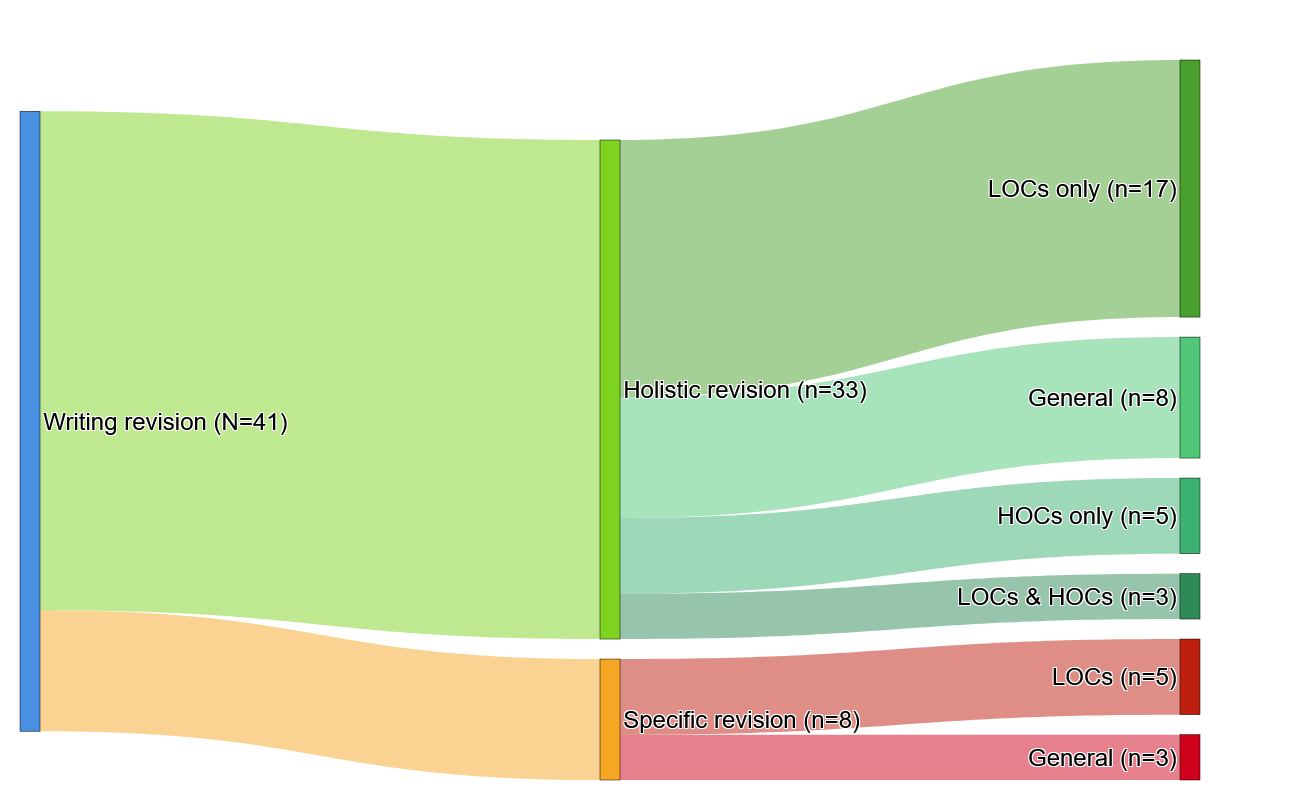
\includegraphics[width=\textwidth]{figure 1.png} \caption{Prompt focus areas in the control group.} \label{fig 1}
    
\end{minipage}
    \source{Created by the authors}
\end{figure}
    


\begin{figure}
    \centering
    
    \begin{minipage}{1\textwidth} 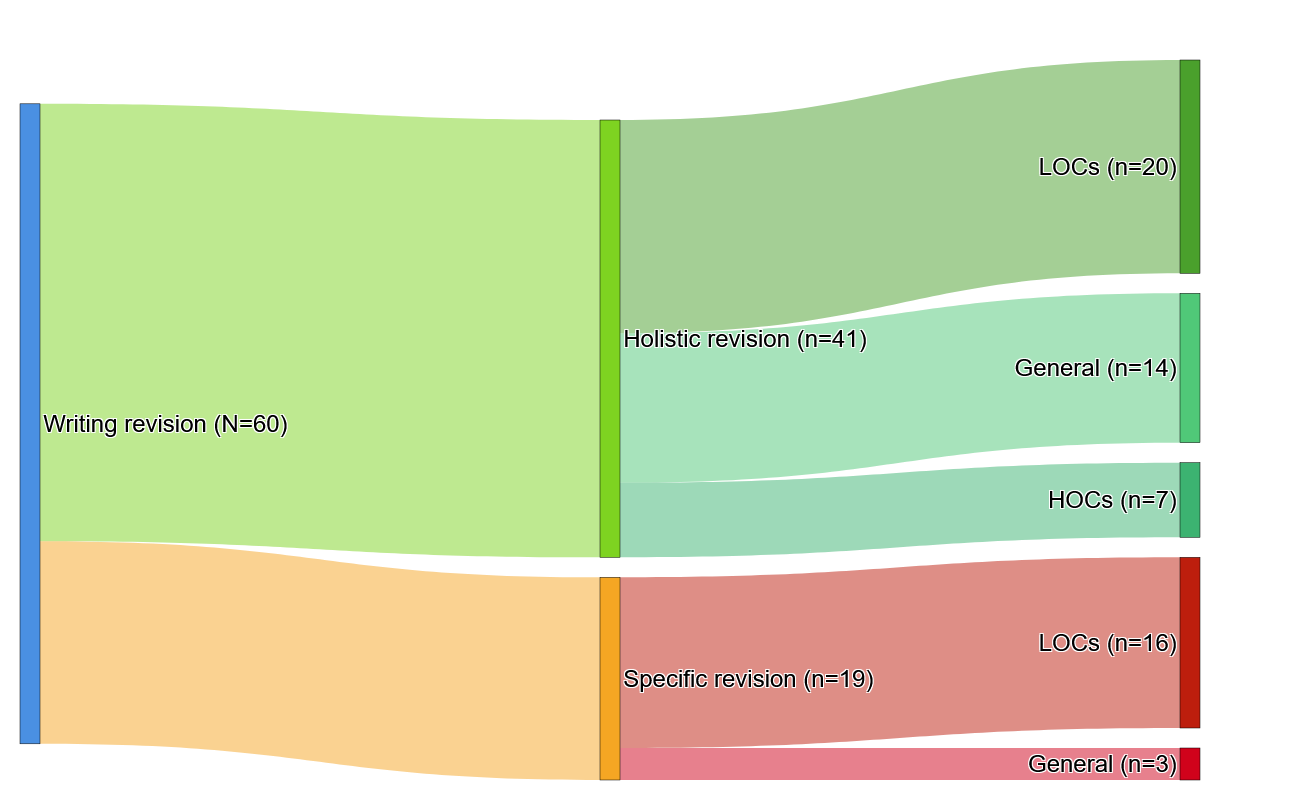
\includegraphics[width=\textwidth]{figure 2.png} \caption{Prompt focus areas in the justification group.} \label{fig 2}
    
\end{minipage}
    \source{Created by the authors}
\end{figure}


Across both groups, lower-level revision requests were predominantly grammar-oriented. In the control group, 21 of the 25 prompts involving LOCs (84\%) explicitly referenced grammar. A similar pattern was observed in the justification group, where 31 of 36 such prompts (86\%) focused on grammar.

Two patterns merit attention. First, in both groups, the majority of prompts either focused on LOCs or represented general revision requests without a specified focus. Combined with the strong emphasis on grammar, this pattern suggests that students may lack metacognitive awareness of revision strategies and therefore tend to default either to nonspecific revision requests or to grammar, which is often the most emphasized aspect of language instruction in Chinese educational contexts.

Second, in the comparison across conditions, the justification group showed a lower proportion of holistic revision prompts. Under the justification requirement, participants produced a greater number of prompts targeting smaller textual units (increasing from 8/41 in the control group to 19/60 in the justification group), although this difference was not statistically significant (19.5\% vs. 31.7\%, $p = .1297$). We further examined prompts that explicitly requested explanation, a feature closely aligned with the justification condition. Although the frequency of such requests increased (from 4/41 to 13/60), the difference again did not reach statistical significance (9.7\% vs. 21.7\%, $p = .0897$). 

Taken together, these findings suggest that requiring justification may encourage learners to engage more deeply with AI-assisted writing revision, attending to details that might otherwise be overlooked, although this effect appears modest rather than pronounced.

\textbf{(v) Alignment between stated objectives, actual prompts, and AI–generated feedback.}

In the control group, of 53 prompts, 14 (26.4\%) failed to accurately convey the participants’ stated objectives. Among these problematic prompts, 11 (78.6\%) were affected by language issues, such as syntactic or lexical errors, while 3 (21.4\%) involved inappropriate prompting strategies. In the justification group, 11 out of 95 prompts (11.6\%) failed to convey the stated objective. Of these, 6 prompts (54.5\%) were affected by language issues, and 5 prompts (45.5\%) were problematic due to inappropriate prompting strategies.

We suggest that many of these problematic prompts may result from participants treating the AI as if it possessed extraordinary comprehension and inferential abilities, expecting it to provide the feedback they had in mind regardless of whether the prompt was linguistically accurate or clearly formulated.

For example, one participant provided only the essay topic without any additional instructions, assuming that the AI would infer the intended objective. Other prompts that were unclear or fragmented included ``A1 and A2 level, any problems in terms of grammar?'' (\emph{a1和a2水平, 语法上有问题吗}) and ``Explain these ten errors in Chinese, briefly present, European Portuguese grammar.'' (\emph{用中文解释这十个错误点，简介，欧洲葡语语法}). Such problematic prompts hinder the AI's ability to provide targeted feedback; however, this issue could be mitigated through greater student understanding of AI capabilities and training in effective prompt design.


Note that students' assumptions about the AI were not entirely unfounded. In the control group, of the 14 problematic prompts, only 2 (15.4\%) ultimately failed to elicit the intended response from the AI (one due to a language issue, one due to a prompting strategy issue). In the justification group, 4 of the 11 problematic prompts (36.4\%) failed to achieve the intended outcome, all of which involved inappropriate prompting strategies.

These findings indicate that the AI's capabilities can partially compensate for suboptimal prompting. Therefore, improving students’ prompting practices may require external guidance, such as instructor intervention, rather than relying solely on trial-and-error interaction with the AI.

\subsection{Accuracy across groups and AI platforms}

Before presenting the comparative results, it is important to note that among the 39 participants, 32 (82\%) used either Doubao or DeepSeek, while use of other models was relatively limited. Because the small sample size of the remaining platforms may reduce data representativeness, the analysis in this subsection and in Subsection \ref{4.3} focuses on the two most widely used models in this study. 

\subsubsection{Comparisons across groups}

First, we compared revision accuracy across the two groups. Revision accuracy was operationalized as the proportion of errors in a text, calculated on a per-word basis.
Three sets of comparisons were conducted:

\begin{itemize}
    \item Doubao accuracy: Control vs. Justification group (3.7\% vs. 6.2\%, $p = 0.0026$)
    \item DeepSeek accuracy: Control vs. Justification group (1.7\% vs. 2.6\%, $p = 0.12$)
    \item Combined accuracy (Doubao + DeepSeek): Control vs. Justification group (3.1\% vs. 5.1\%, $p = 0.0031$)
\end{itemize}

Across all comparisons, accuracy was consistently higher in the control group (i.e., the error rate was lower). Although the accuracy difference for DeepSeek alone did not reach statistical significance, the differences observed for Doubao and for the two models combined were statistically significant.

These findings suggest that requiring justification during the revision process does not improve and may in fact reduce the accuracy of AI-assisted revisions. This effect may stem from model limitations, since generating revisions and explanations simultaneously could lower output quality. Alternatively, it may be related to human factors. The requirement to justify changes could increase cognitive load, potentially reducing prompt quality and, as a result, revision quality. The underlying mechanism remains unclear based on the current data and warrants further investigation in future research.

\subsubsection{Comparisons across AI platforms}
In this subsection, we compare revision accuracy between the two AI platforms. Three sets of comparisons were conducted:

\begin{itemize}
    \item Doubao vs. DeepSeek in the control group: 3.7\% vs. 1.7\%, $p = 0.0042$
    \item Doubao vs. DeepSeek in the justification group: 6.2\% vs. 2.6\%, $p = 0.0011$
    \item Doubao vs. DeepSeek combining data from both groups: 4.8\% vs. 2.1\%, $p = 0.0001$
\end{itemize}

Across all comparisons, DeepSeek consistently produced lower error rates than Doubao. These differences were statistically significant in every case, indicating that platform choice had a substantial impact on revision accuracy. Under this learner-prompting condition, DeepSeek appears to be more effective than Doubao in helping participants perform accurate revisions. The differences in revision accuracy between the models will be further investigated under a more controlled experimental setting using researcher-designed prompts in Section \ref{4.3}.

\subsection{Effects of research-designed prompts}\label{4.3}

In this subsection, we compare revision accuracy under different research-designed prompts across the two AI platforms. The experiments are conducted under the control condition, given its higher accuracy relative to the justification condition.

For DeepSeek, the error rates under different settings were as follows: RaR (1.3\%), Control (1.7\%), Basic (2.3\%), and Role prompting (3.4\%). Pairwise comparison results are summarized in Table \ref{tab1}.

\begin{table}[htpb]
\centering
\begin{threeparttable}
\caption{Pairwise comparisons of DeepSeek error rates across prompting conditions.}
\label{tab1}
\begin{tabular}{lccccc} 
\hline
Method         & Error Rate (\%) & vs. Control & vs. Role & vs. Basic & vs. RaR  \\ 
\hline
Control        & 1.7             & —           & *        & •         &         \\
Role Prompting & 3.4             &            & —        &          &         \\
Basic          & 2.3             &            & *        & —         &         \\
RaR            & 1.3             & •           & *        & *         & —        \\
\hline
\end{tabular}
\source{Created by the authors.}
\notes{* indicates the row method is significantly better (lower error rate) than the column method ($p < 0.05$); • indicates the row method is numerically better but not statistically significant.}
\end{threeparttable}
\end{table}


Pairwise comparisons show that RaR achieved the lowest overall error rate, significantly outperforming both Basic and Role Prompting. Although RaR had a lower error rate than Control, this difference was not statistically significant. Control significantly outperformed Role Prompting and showed a numerical—but not statistically significant—advantage over Basic . Basic, in turn, significantly reduced errors compared to Role Prompting.


For Doubao, the error rates under different prompting conditions were as follows: RaR (1.6\%), Basic (1.7\%), Role Prompting (2.5\%), and Control (3.7\%). Pairwise comparisons are summarized in Table \ref{tab2}.

\begin{table}[htpb]
\centering
\begin{threeparttable}
\caption{Pairwise comparisons of Doubao error rates across prompting conditions.}
\label{tab2}
\begin{tabular}{lccccc} 
\hline
Method         & Error Rate (\%) & vs. Control & vs. Role & vs. Basic & vs. RaR  \\ 
\hline
Control        & 3.7             & —           &          &           &          \\
Role Prompting & 2.5             & •           & —        &           &          \\
Basic          & 1.7             & *           & *        & —         &          \\
RaR            & 1.6             & *           & *        & •          & —        \\
\hline
\end{tabular}
\source{Created by the authors.}
\notes{* indicates the row method is significantly better (lower error rate) than the column method ($p < 0.05$); • indicates the row method is numerically better but not statistically significant.}
\end{threeparttable}
\end{table}

Pairwise comparisons show that RaR achieved the lowest error rate, followed closely by Basic. Although RaR performed slightly better than Basic, this difference was not statistically significant. Both RaR and Basic significantly outperformed Control and Role Prompting. While Role Prompting yielded a lower error rate than Control, this difference was not statistically significant.

The results across the two AI platforms suggest that among the three researcher-designed prompts, RaR achieved the highest accuracy, followed by Basic, while Role Prompting performed the worst. This indicates that the effectiveness of prompt engineering cannot be assumed in advance, as prompting strategies that perform well in one task context may not necessarily improve performance in another and may even perform worse than a simple baseline or naïve prompting approach.

From an instructional perspective, this suggests that effective teaching of prompt engineering requires emphasizing the sensitivity of large language models to variations in prompt design and the importance of iterative testing. Rather than assuming that a single prompting technique will consistently produce optimal results, students should be encouraged to experiment with diverse prompting strategies, assess their performance empirically, and refine them based on observed outcomes.

\section{Discussion and conclusion}\label{sec5}

The present study offers a detailed empirical examination of authentic learner prompting behavior in AI-assisted revision of L2 Portuguese writing, conducted with Chinese university students in Macau. The findings paint a consistent picture of relatively immature prompting practices: strongly anthropomorphic interpersonal prompting style, heavy reliance on generic or lower-level (especially grammar-focused) requests, and frequent misalignment between intended objectives and actual prompts. These patterns mirror prior work \cite{hwang2024exploring,KNOTH2024100225,zamfirescu2023johnny}, confirming that unsophisticated prompting is a common feature of novice LLM users.

The task manipulation requiring justification for every modification proved to be a simple yet powerful intervention. It significantly increased interaction turns, raised the proportion of explanation-seeking prompts, and shifted learners toward more focused, smaller-unit revisions. These behavioral changes demonstrate that even minimal task-design scaffolding can promote deeper engagement with AI feedback, moving students away from passive ``copy-paste’’ revision toward genuine inquiry and understanding. This represents a key pedagogical insight: instructors can enhance human–AI interaction simply by requiring students to justify their revisions. Similarly, prompting for explanations in other learning activities may encourage more reflective engagement with AI tools.

At the same time, the persistent immaturity of prompting across both conditions, including vague holistic requests, overemphasis on grammar, and misalignment due to linguistic or strategic shortcomings, highlights the necessity of explicit guidance in prompt engineering and AI literacy \cite{hwang2023prompt}. Without such guidance, students are likely to receive highly variable feedback and forfeit much of the potential learning benefit. Educators should therefore transition from merely tolerating AI use to actively teaching effective prompting strategies, and designing tasks that reward explanation-seeking over blind acceptance.

On revision accuracy, this study establishes a realistic and encouraging benchmark for AI-assisted L2 writing under authentic, untrained student prompting. From an original learner text with an error rate of approximately 19.1\%, final revisions achieved error rates of 1.7–6.2\%, depending on platform and condition, representing an error reduction of 68–91\%. Even in the least favorable condition, AI assistance delivered substantial linguistic improvement. These results were obtained with students’ preferred (Chinese-interface) tools and without any prompt training, demonstrating that current LLMs already provide substantial pedagogical value in real-world settings despite remaining imperfections. We should firmly reject the perfectionist notion that AI must be error-free before it can be educationally useful; the evidence shows it is already transformative when used even naively.

Researcher-designed prompts further illustrated the sensitivity of LLM performance to prompting. The Rephrase-and-Respond technique achieved the lowest error rates (1.3–1.6\%), while the widely recommended role-prompting approach performed worst on DeepSeek and only marginally better than student prompts on Doubao. These findings underscore that prompt engineering is highly context-dependent and techniques cannot be assumed universally effective. Instruction should therefore emphasize iterative experimentation rather than rote application of supposed best practices.

In conclusion, this study positions AI not as a replacement for teachers but as a powerful learning partner, particularly valuable for low-resource L2s like Portuguese in Macau, where its accessibility, immediacy, and infinite patience address precisely the gaps left by limited native-speaker contact. Realizing this potential, however, demands deliberate pedagogical intervention: systematic teaching of prompting strategies, task designs that mandate justification and explanation-seeking, and cultivating a critical awareness that AI is not merely a tool for outsourcing. When students learn to interrogate rather than simply accept AI suggestions, the synergy of human reflection and machine capability can profoundly enhance second-language writing development.

Although the study is limited by its relatively small sample (n = 39 after exclusions), focus on a single learner composition, and specific sociocultural context, the convergence of findings with L2 English studies suggests broad generalizability of both the problems identified and the effectiveness of the proposed interventions. Future research should employ larger and more diverse samples, longitudinal designs to track development over time, comparisons across proficiency levels, and exploration of additional task interventions. Nevertheless, the present results provide robust empirical grounding for immediate pedagogical action: educators can (and should) begin systematically guiding students toward more critical, reflective, and effective use of AI in writing development today.


\printbibliography\label{sec-bib}


%full list: conceptualization,datacuration,formalanalysis,funding,investigation,methodology,projadm,resources,software,supervision,validation,visualization,writing,review
\begin{contributors}[sec-contributors]
\authorcontribution{Mu You}[conceptualization,datacuration,formalanalysis,writing,review]
\authorcontribution{Jing Zhang}[investigation,datacuration,formalanalysis,review]
\authorcontribution{Chunhui Lu}[conceptualization,investigation,methodology,datacuration]
\authorcontribution{Ana Cristina Ferreira de Almeida Rodrigues Alves}[methodology,datacuration,formalanalysis,review]
\authorcontribution{Jiaxu Zuo}[investigation,software,visualization]

\end{contributors}



\begin{dataavailability}
\txtdataavailability{dataonly} % options: dataavailable, dataonly, databody, datanotav, nodata
\end{dataavailability}

\appendix
\section{Materials}
\label{app:materials}

\textbf{Essay prompt:} \\
Hoje em dia, as atividades das crianças nos tempos livres são muito diferentes daquelas no passado. Escreva um texto, com aproximadamente 100 palavras, sobre o que costumava fazer nos seus tempos livres quando era criança e compare a sua infância com a vida das crianças nos dias de hoje.\\

\noindent\textbf{Composition:} \\
Quando eu era pequena, vivia na cidade. Por isso, não tinha muito lugar para brincar com os amigos. Como não tínhamos rio, podíamos brincar no jardim ao lado da minha casa. Além de brincar, costumávamos jogar ténis de mesa e correr pela calçada. Que tempo feliz e interessante! Quando o tempo não estava bom, eu ficava em casa, lia livros ou via televisão nos tempos livres. Mas o que eu mais gostava era viajar com os meus pais nas férias.  

A infância das crianças nos dias de hoje é muito diferente da minha. Eu não tinha um telemóvel, mas quase todas as crianças hoje têm um. E elas gostam muito de jogar com ele. Conheço uma criança, filha de um colega do meu pai, que não faz outra coisa além de jogar jogos no telemóvel todos os dias. Acho que jogar no telemóvel é mais entediante do que brincar no jardim ou ler livros. Também penso que esse tipo de infância é prejudicial para as crianças nos dias de hoje.\\



\noindent\textbf{Part 1 of the task instructions for the control group:} \\

任务1

你将得到一份葡语作文，请使用AI对该作文进行改写和提升。之后你需要按我们提供的指引将修改后的作文提交，并逐句解释修改的理由。任务1完成后，请举手示意。

注意事项:
1.	请完整保留你与AI的所有对话记录。这些记录不仅是研究的重要材料，也有助于我们在后续课程中更有针对性地帮助你提升AI使用技能。
2.	请合理安排时间，尽可能全面地修改作文里所有需要改进的部分。

Task 1

You will receive a Portuguese composition. Please use AI tools to revise and improve it. Afterwards, you need to submit the revised composition according to the instructions we provide, and explain the rationale for each modification sentence by sentence.
Once you have completed Task 1, please raise your hand.

Notes:
1.	Keep a complete record of all your interactions with AI. These records are essential for research purposes and will also help us provide more targeted support in future lessons to strengthen your prompting skills.
2.	Revise the composition thoroughly, addressing all parts of the text that require improvement.\\

\noindent\textbf{Part 2 of the task instructions for the control group:} \\

请打开“AnswerSheet.docx”，按照以下指引完成任务2。

•	请将修改完成的作文复制到“A”下空白处。

•	请将你与AI的*所有*对话记录完整地复制到“B”区，并解释每个指令的目的。

示例：
指令1：你能帮我改下这篇作文吗？
目的：我想让AI帮我全面地修改作文
AI回答：[…]

指令2：[…]，这句话是什么意思，还能怎么改
目的：我不理解这句话，想让AI解释清楚，同时还想看看还有什么改法
AI回答：[…]

指令3：[…] 这个语法我不太会，请你逐步解释，并提供示例
目的：我对这个语法有点不熟悉，想让AI更清楚地解释一下
AI回答：[…]


注意事项
1.	请完整地复制你与AI的所有对话记录，不要有遗漏。
2.	任务完成后，请举手示意。

Please open “AnswerSheet.docx” and complete Task 2 according to the following instructions.

• Copy the revised essay into the blank space under “A”.

• Copy the entire record of your conversation with the AI into section “B” and explain the purpose of each prompt.

Example:

Prompt 1: Can you help me revise this essay?
Purpose: I want the AI to comprehensively improve my essay.
AI Response: […]

Prompt 2: What does this sentence mean, and how else could it be rewritten?
Purpose: I didn’t understand this sentence and wanted the AI to explain it clearly, while also showing me alternative ways to revise it.
AI Response: […]

Prompt 3: I’m not very familiar with this grammar point — please explain it step by step and provide examples.
Purpose: I was unsure about this grammar and wanted the AI to clarify it thoroughly.
AI Response: […]

Notes:
1.	Copy all your dialogue with the AI completely. DO NOT OMIT ANY PART.
2.	When you have finished the task, please raise your hand to signal completion.\\


\noindent\textbf{Part 1 of the task instructions for the justification group:} \\

任务1

你将得到一份葡语作文，请使用AI对该作文进行改写和提升。之后你需要按我们提供的指引将修改后的作文提交，并逐句解释修改的理由。任务1完成后，请举手示意。

注意事项:
1.	请完整保留你与AI的所有对话记录。这些记录不仅是研究的重要材料，也有助于我们在后续课程中更有针对性地帮助你提升AI使用技能。
2.	请合理安排时间，尽可能全面地修改作文里所有需要改进的部分。

Task 1

You will receive a Portuguese composition. Please use AI tools to revise and improve it. Afterwards, you need to submit the revised composition according to the instructions we provide, and explain the rationale for each modification sentence by sentence.
Once you have completed Task 1, please raise your hand.

Notes:
1.	Keep a complete record of all your interactions with AI. These records are essential for research purposes and will also help us provide more targeted support in future lessons to strengthen your prompting skills.
2.	Revise the composition thoroughly, addressing all parts of the text that require improvement.\\

\noindent\textbf{Part 2 of the task instructions for the control group:} \\

请打开“AnswerSheet.docx”，按照以下指引完成任务2。

•	请将修改后的作文复制到“A”下空白处。

•	请将你与AI的*所有*对话记录完整地复制到“B”区，并解释每个指令的目的。

示例：
指令1：你能帮我改下这篇作文吗？
目的：我想让AI帮我全面地修改作文
AI回答：[…]

指令2：[…]，这句话是什么意思，还能怎么改
目的：我不理解这句话，想让AI解释清楚，同时还想看看还有什么改法
AI回答：[…]

指令3：[…] 这个语法我不太会，请你逐步解释，并提供示例
目的：我对这个语法有点不熟悉，想让AI更清楚地解释一下
AI回答：[…]

•	请你在“C”区逐句解释修改的理由。


注意事项
1.	请完整地复制你与AI的所有对话记录，不要有遗漏。
2.	任务完成后，请举手示意。

Please open “AnswerSheet.docx” and complete Task 2 according to the following instructions.

• Copy the revised composition into the blank space under “A”.

• Copy the entire record of your conversation with the AI into section “B” and explain the purpose of each prompt.

Example:

Prompt 1: Can you help me revise this essay?
Purpose: I want the AI to comprehensively improve my essay.
AI Response: […]

Prompt 2: What does this sentence mean, and how else could it be rewritten?
Purpose: I didn’t understand this sentence and wanted the AI to explain it clearly, while also showing me alternative ways to revise it.
AI Response: […]

Prompt 3: I’m not very familiar with this grammar point — please explain it step by step and provide examples.
Purpose: I was unsure about this grammar and wanted the AI to clarify it thoroughly.
AI Response: […]

•	In section “C”, provide the reasons for each revision sentence by sentence.

Notes:
1.	Copy all your dialogue with the AI completely. DO NOT OMIT ANY PART.
2.	When you have finished the task, please raise your hand to signal completion.\\











\end{document}

